\section{ER-Diagrammer}
\begin{frame}{Entity-Relationship Diagrammer}
    \begin{itemize}[<+->]
        \item Grafisk versjon av en database
        \item Identifikasjon av entiteter
        \item Identifikasjon av sammenheng mellom entiteter
    \end{itemize}
\end{frame}

\subsection*{Kardinalitet}
\begin{frame}{Kardinalitet}
\begin{columns}
    \begin{column}{0.48\textwidth}
\begin{tikzpicture}[every node/.style={font=\scriptsize}]
    \draw[mone-,thick] (0,0) -- node[above]{eksakt 1}node[below]{(1,1)} (5,0);
    \draw[mmany-,thick] (0,-1) -- node[above]{minst en}node[below]{(1,n)} (5,-1);
    \draw[oone-,thick] (0,-2) -- node[above]{opptil en}node[below]{(0,1)} (5,-2);
    \draw[omany-,thick] (0,-3) -- node[above]{ 0, 1 eller mange}node[below]{(0,n)} (5,-3);
    \end{tikzpicture}
 	\end{column}
    \begin{column}{0.48\textwidth}
\begin{tikzpicture}[every node/.style={font=\scriptsize}]
    \draw[mone-mone,thick] (0,0) -- node[above]{one-to-one}node[below]{} (5,0);
    \draw[mone-omany,thick] (0,-1) -- node[above]{one-to-many}node[below]{} (5,-1);
    \draw[omany-omany,thick] (0,-2) -- node[above]{many-to-many}node[below]{} (5,-2);
    \end{tikzpicture}
 	\end{column}
\end{columns}
    
\end{frame}

\begin{frame}{Eksempler}
    %\begin{itemize}
        %\item<1-1> Person - Fødselsby
        %\item<2-> Person (0,n) - (1,1) Fødselsby
        %\item<3-3> Kunde - Produkt
        %\item<4-> Kunde (0,n) - (0,n) Produkt
        %\item<5-5> Medarbeider - Prosjekt
        %\item<6-> Medarbeider (1,n) - (1,1) Prosjekt
        %\item<7-7> Land - Hovedstad
        %\item<8-> Land (1,1) - (1,1) Hovedstad
        %\item<9-9> Film - Regissør
        %\item<10-> Film (0,n) - (1,n) Regissør
        
    %\end{itemize}
\begin{tabular}{l|l|l}
    Tabell & Kardinalitet & Navn\\\hline\pause
    Person - Fødselsby & (0,n) - (1,1) & one-to-many\\\pause
    Kunde - Produkt & (0,n) - (0,n) & many-to-many\\\pause
    Medarbeider - Prosjekt & (1,n) - (1,1) & one-to-many\\\pause
    Land - Hovedstad & (1,1) - (1,1) & one-to-one\\\pause
    Film - Regissør & (0,n) - (1,n) & many-to-many
    \end{tabular}
\end{frame}

\begin{frame}{}
    \begin{figure}
        \centering
        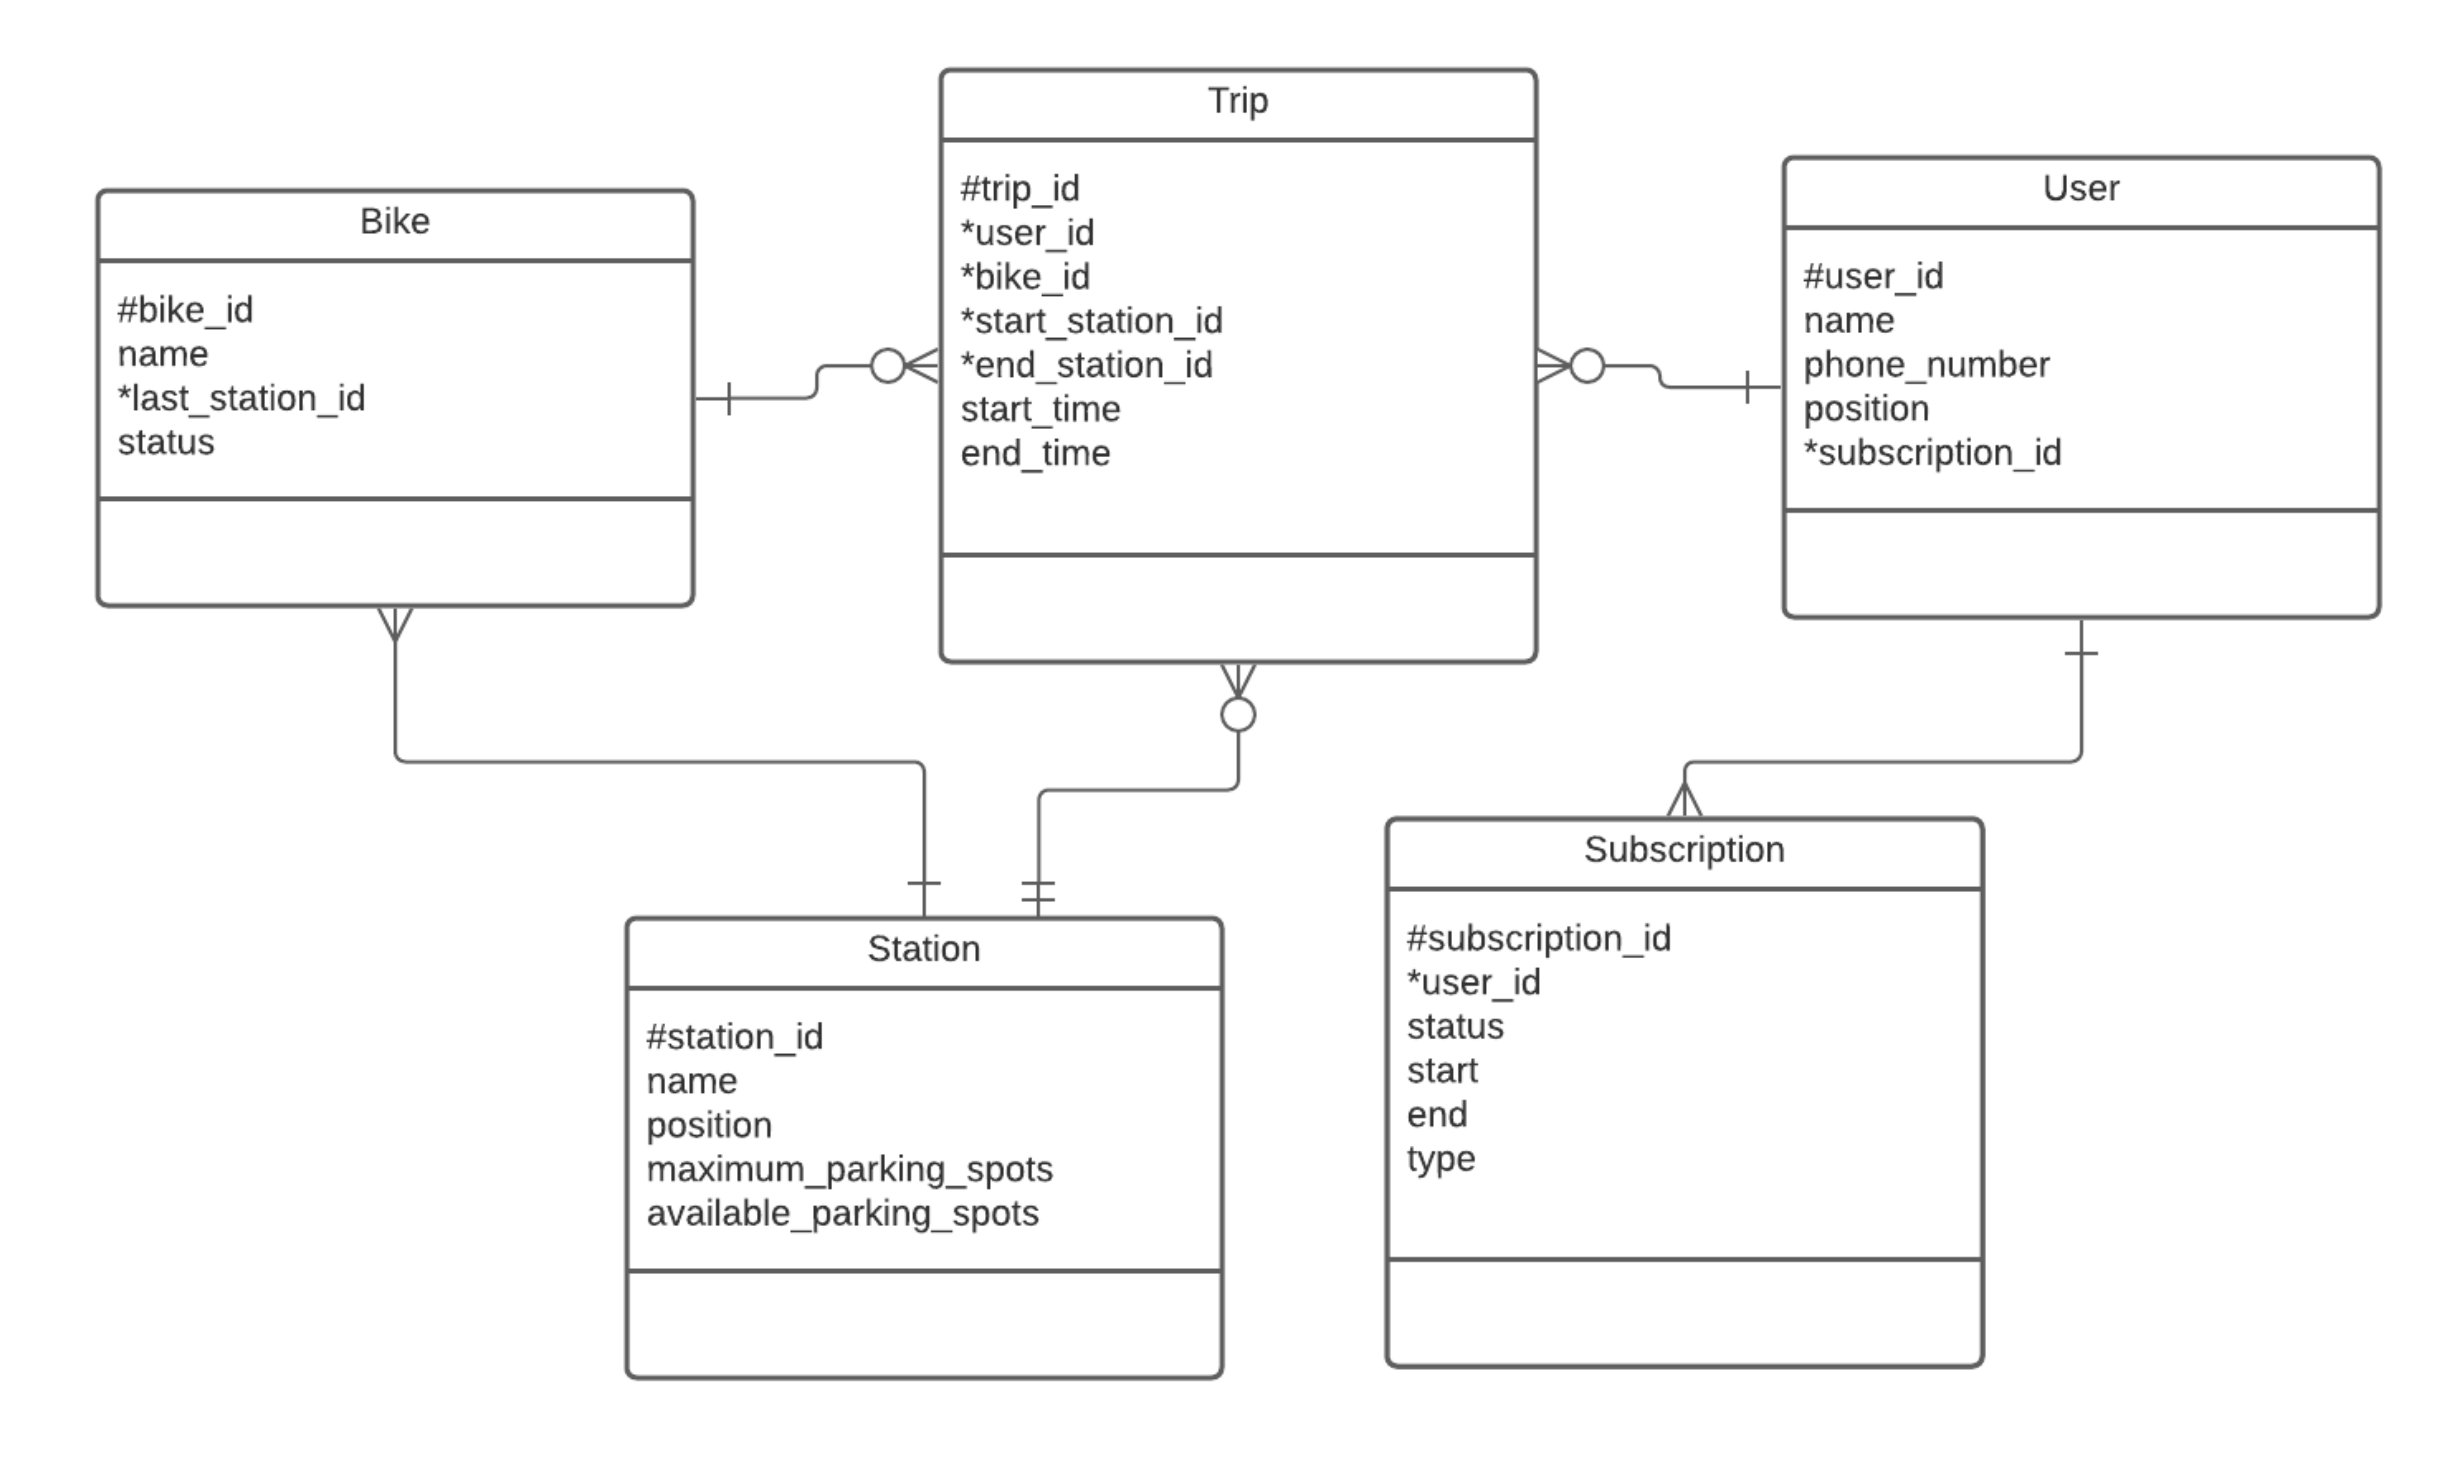
\includegraphics[height = 4.9cm]{images/erdiagram.png}
        \caption{Eksempel ER-diagram fra oblig 2}
        \label{fig:erdiagram}
    \end{figure}
\end{frame}

\subsection*{Spørretid}
\begin{frame}{Spørsmål?}
    \begin{figure}
        \centering
        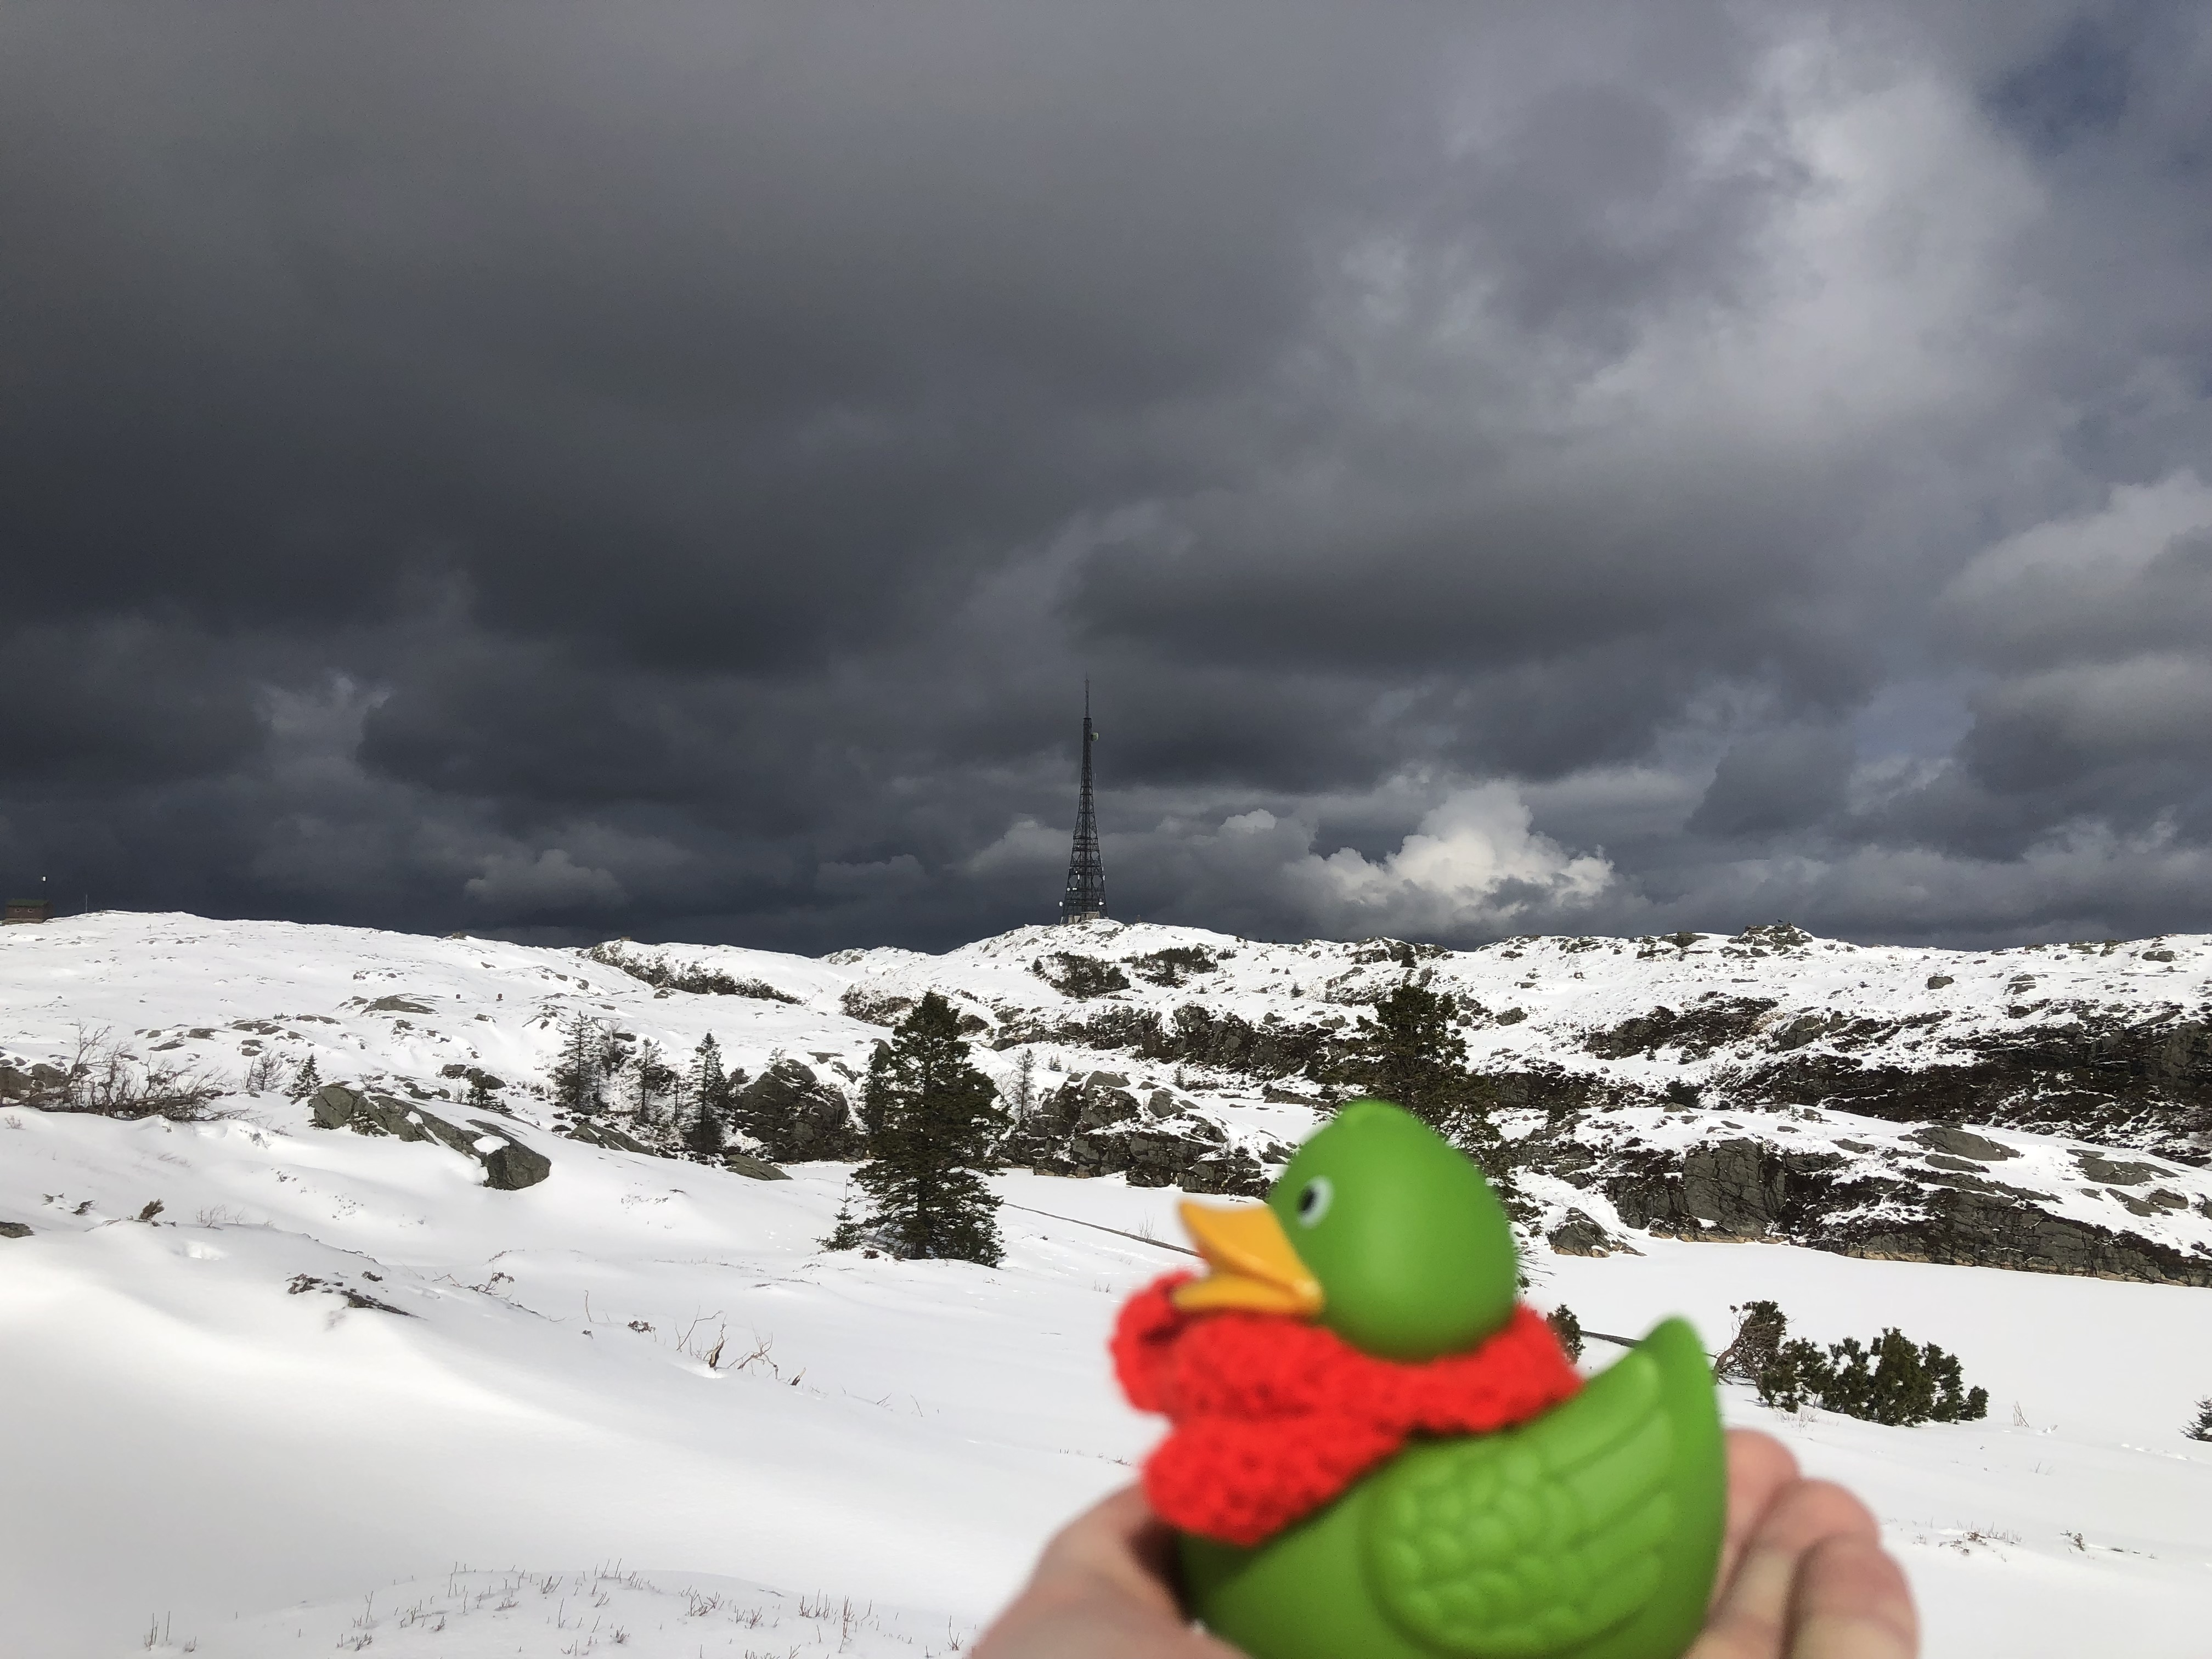
\includegraphics[height = 4.9cm]{images/guillaume6.jpg}
        \caption{Guillaume på Blåmanen}
        \label{fig:guillaume6}
    \end{figure}
\end{frame}